\section{Design and Implementation}
\label{sect:apner_architecture}
As previously mentioned, our main goal is designing polyNER is to slash labeling costs by reducing the time and effort spent by experts to generate training data. 
Rather than labeling entire documents and phrases, annotators label proposed candidate entities to be classified.
%\logan{What is downstream in this metaphor? I also don't think it is a needed detail}\roselyne{ok, removed, it stemmed from the idea in my head about mentioning that our labels can be used by Hong, and others later, picked up from snuba, but probably can be emphasized better or elsewhere}.
Earlier results show that with two hours of labeling we can achieve
precision or recall (but not yet both) on par with state-of-the-art domain specific software, by selecting an ensemble of classifiers for discrimination~\cite{tchoua2019polyner}. %\loganfussingaboutrecallandprecision \roselyne{noted, will specify in results that we also use ROC and PR curves}

Here, we refine polyNER components and incorporate active learning with different sampling strategies in order to further improve performance.
PolyNER uses word representations and minimal domain knowledge (a few
seed entities) to produce a small set of candidates for expert labeling;
labeled candidates are then used to train named entity word vector classifiers.
We integrate an active learning loop into polyNER's architecture to incrementally improve classifier performance.

In order to explore whether the use of word vector coordinates as features can accelerate the learning process,
we define and compare three alternative sampling strategies: a random strategy that we use as a baseline,
and two NLP-based filtering methods. 
%\ian{Are the three strategies all an integral part of polyNER, or are they alternatives that we compare? Unclear. I reworded to say they are alternatives, is that right?}\roselyne{Yes to alternatives that we compare.}
We also apply these methods against two different candidate pools, 
one set of unlabeled nouns and another set of approximately labeled nouns deemed \textit{similar} to commonly used known entities from our corpus.
%\ian{The candidate pool reference is confusing to me because in the text that follows you seem to refer to just one
%pool, the ``NLP-filtered candidates."}\roselyne{I specifically describe two pools, the NLP filtered, and the distance NLP-filtered, perhaps too wordy?}
We describe our sampling strategies and approximate labeling in more details in this section.
% for maximum entropy uncertainty sampling, which we describe in this section.
%\logan{We have mentioned these two different pools twice now, but haven't given a hint as to what they are. I think we should describe them succinctly here.}\roselyne{Done I think}
The general architecture of polyNER is illustrated in Figure~\ref{fig:architecture}.
We also describe the labeling process, and the training and testing configuration for our word vector classifiers in the active learning loop. 

\begin{figure*}[!t]
{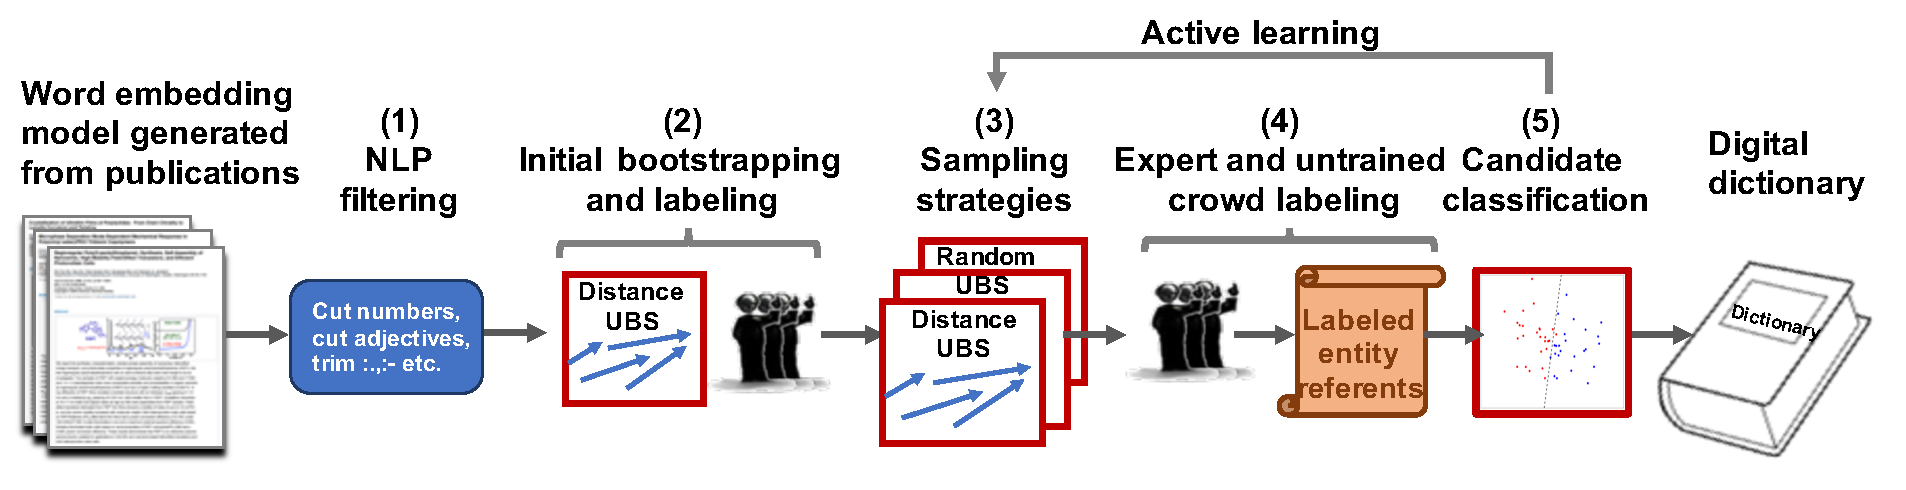
\includegraphics[width=\textwidth]{figures/architecture.pdf}}
\caption{\label{fig:architecture} PolyNER system showing the different phases of polyNER including the NLP-filtering step, the initial sampling and the newly integrated active learning loop to classify scientific named entities. 
%\ian{(1) It is really important to be consistent in how your refer to things. Here, the figure says ``Bootstrapping and Initial Labeling" for (1), but the caption says ``initial sampling and labeling.'' Pick one and use it consistently. (2) You are inconsistent in capitalization. (3) The caption mostly repeats the labels in the figure, which seems redundant.
%It could be higher level.}
	%\logan{Should we differentiate between the "initial sampling" strategy done to bootstrap our training set and the "active learning sampling" strategy used to identify the next things to label? Mixing the two up is going to confuse people}\roselyne{OK will adapt the rest of the text and section titles too.}
}
\end{figure*}

\subsection{NLP-Filtering}\label{sec:filter}
%\subsubsection{Word Embedding Model}
%\logan{Why is this titled "Word Embedding Model" and you start by describing a classifier?}
%We hypothesize that we can implement a classifier, which can detect word vectors for polymers based on their context. 
%\logan{This is the only section that you start with a "hypothesis"}\roselyne{ok removing this and moving section}
%\logan{Where is this section in F\ref{fig:architecture}?}
%We generate an unsupervised word embedding model using out entire corpus and train classifiers on vector representations using labels generated via the active learning(step 3 of Figure~\ref{fig:current}).
%Finally, in step 4, we test our classifiers against all the NLP-filtered words from the test corpus, as shown on Figure~\ref{fig:current}.

%\logan{Make section labels line up with the names in the figures}
First, we define an
NLP filtering preprocessing step to filter out
string
%\ian{Maybe the wrong term, as the first example is ``polyethylene;'', which is not a ``word'' but a string?}
 in scientific publications that are unlikely to be polymer referents. 
%In other words, we remove obvious non-candidates.
First, we remove
unwanted characters (e.g. `:', `.', `,', `:', `-') from the beginning and the end of each
candidate and eliminate numbers (including numbers followed by common units).
This step allows us to recognize, for example, ``polyethylene;'' and eliminate it as yet another unique (erroneous) candidate. 
%\ian{I can't tell what you are saying in the preceding. Can we simply say, ``thus, for example,
%we can eliminate ``polyethylene;'' as a string distinct from ``polyethylene.'' [I am not sure if I have worded this
%right.]}\roselyne{not sure I understand that better, but I think I can rephrase}
Hypothesizing that names of scientific entities will not, in general, be English
vocabulary words, we remove words found in the SpaCy dictionaries
of commonly used English words~\cite{choi2015depends}. (We manually remove common polymer
names, such as polystyrene and polyethylene, from the dictionaries.) 
We also use
SpaCy's part-of-speech tagging functionality to remove non-nouns.  
Finally, we remove plurals (e.g.,
polyamides, polynorbornenes), as they can represent polymer family names.
Note that these steps are generalizable and applicable to multiple science fields.
%\logan{2 is the only number that does not start with "We remove." Should you make this a bulleted list?}\roselyne{Good point, but then this is hardly a section I think, I will try and see how it looks. Also some of the bullet text is short and some is long. e.g. numbers vs, entire sentence.}
We refer to the set of words that result when these filtering operations are applied to our corpus (the output of step 1 in Figure~\ref{fig:architecture}) as the \emph{NLP-filtered candidates}.


\subsection{Initial Labeling}
While the previous step%\ian{Should this be singular?}
 reduce the numbers of candidates and the imbalance of the dataset (target vs.\ non-target entity ratio), 
 there still remains a relatively large pool of potential candidates from which entities are to be selected.
In our experience, the ratio of polymers-to-non-polymers in NLP-filtered words in publications is $\sim$5\%.\ian{I don't think that a ratio can be a percentage. You may mean ``only 5\% of NLP-filtered words are polymer names.}
In order to avoid presenting experts with mostly negative examples, hindering meaningful classification,
we attempt to boost the number of polymer entities in the first batch of candidates to be annotated by using word vector similarity metrics between candidates and commonly used known entities as observed in a subset of publications or as suggested by experts.
We discuss this distance metric in more details below.
\ian{You refer to similarity metrics in one sentence and distance metric in the next. Be consistent!}\roselyne{Leave this here to check everywhere}
%Candidate batch sizes are determined based on labeling time estimates and availability of expert curators.
Based on preliminary experiments, we set the size of each batch of strings to be labeled to 200, 
or about an hour of expert time.

\subsection{Sampling Strategies}
%While the previous steps reduces the numbers of candidates and the imbalance of the dataset (target vs. non-target entity ration), there still remains a relatively large pool of potential candidates to select entities from.
%In order to achieve higher classification accuracy\textemdash
%by decreasing the number of potential false positives (candidates incorrectly identified as targets by our classifier)
%\textemdash we want to carefully select examples to be labeled by experts.
%\logan{Why is labeling "false positives" bad?}\roselyne{It just takes more time from the expert, also we can't give the expert only negative examples.}
We implement three sampling strategies, which we refer to as \textit{Random}, \textit{Uncertainty-Based Sampling (UBS)} and \textit{Distance Uncertainty-Based Sampling (Distance UBS)}.
We apply each of these strategies to our NLP-filtered candidates to determine which candidates to label.
%Based on preliminary experiments, we set the size of batches of strings to be labeled to 200 or about an hour of expert time.
%\logan{As my comment in F\ref{fig:architecture}, we have two different kinds of sampling strategies and I think we should describe them separately. What do you think?}\roselyne{I'm separating the initial sampling and adding it to the figure}

\subsubsection{Random Strategy using NLP-Filtered Candidates}
In the first strategy, we randomly select 200 out of the pool of unlabeled NLP-filtered candidates from the entire corpus of publications.
Note that the imbalance between polymers and other NLP-filtered \textit{tokens} (words or space separated strings)  is still significant (less than 5\% in our test set).
%We exclude tokens included in our test set.\ian{I have no idea what the preceding text is saying. What does it mean to have an imbalance with things that do not exist?
%Could this paragraph simply be, ``As a baseline, we will present results for a random selection strategy,
%in which 200 candidates are selected at random from the NLP-filtered candidates.''}\roselyne{It's missing dictionary, that do not exist in the dictionary}
%\ian{Separate issue: as far as I know, you have not introduced the concept of a test set, so the reference to test set is confusing.}

\subsubsection{Uncertainty-Based Sampling using NLP-Filtered Candidates (UBS)}
Our second strategy applies maximum entropy sampling to the NLP-filtered candidates. % from the full corpus of documents used in the random strategy.
%\logan{Same pool}
As previously mentioned, maximum entropy selection is an uncertainty sampling method that
identifies data points for which a classifier predicts outcomes that lie near the decision boundary 
between classes. 

%\ian{I don't understand the next text. Could we write, 
%``For example, when predicting whether or not a word vector represents a polymer, 
%maximum entropy arises when the classifier assigns equal probability to the polymer and not-polymer cases.''}
For example, when predicting whether or not a word vector represents a polymer, maximum entropy arises when the classifier assigns equal probability to the polymer and not-
polymer cases.
As we have two classes, this equal probability is 0.5.
%For example, in our case, when predicting whether or not a word vector represents a polymer, 
%the classifier assigns equal probability to either case.
%\ian{Can we say, ``As we have two classes" rather than ``in the binary case"?}
%In the binary case, probabilities range from 0 to 0.5. 
%\ian{Why can't you have a probability of 1, for say ``polystyrene''?}\roselyne{You're right, you can have that, and the text is confusing, if you you have a probability of 1, then |1-0.5| gives you 0.5 and this will not be considered as a confusing example, the examples with probability p with |0.5-p| close to 0 are the ones considered confusing} 
Therefore, we predict outcome for all our NLP-filtered candidates and obtains a probability $p$ for each data point. We compute a list of $0.5-p$ values for all unlabeled data and sort the list in ascending order.
Points with scores closest to $0$ are most uncertain.
We select the first 200 entries from this ordered list to be labeled by experts.

\subsubsection{Uncertainty-Based Sampling using NLP-Filtered Distance Candidates (Distance UBS)}
Our second strategy selects NLP-filtered candidates that are 
deemed to be most similar to seed entities as determined by vector similarity measures.
%\ian{It is confusing that for the first two strategies, you refer to them as strategies, and here you switch to talking about a pool. (Further adding to confusion is that earlier you said you had two pools. Here you refer to the ``third pool.'') Can we say, rather: ``Our second strategy selects NLP-filtered candidates that are 
%deemed to be most similar to seed entities as determined by vector similarity measures.
%The intuition behind this strategy..."}\roselyne{This is an error, there is no third pool}
The third pool is composed of NLP-filtered candidates deemed to be most similar to seed entities as determined by vector similarity measures.
The intuition behind generating this pool of candidates is to increase the likelihood that a candidate is a target referent (name, acronym, synonym, etc.) by comparing its vector to that of a known entity.
Our goal is to determine whether polymers are used in a consistent context that can be used to detect and classify their corresponding context-aware vectors.
For example, the polymer name ``polystyrene'' in a sentence ``The
melting point of polystyrene is ...'' suggests that X may also be a polymer in the
sentence ``The melting point of X is ...''.

%\ian{I added a new paragraph here because I feel that readability suffers due to long paragraphs.}

A word embedding method \ian{You referred to ``vector similarity" but then switch to talking about word embedding.
Maybe say ``We use word embedding methods to obtain the vectors that we use for determining similarity.''} 
maps each word
in a sentence or document to a vector in an n-dimensional real vector space
based on the linguistic context in which the word appears. (This mapping may
be based, for example, on co-occurrence frequencies of words.) 
We can then
determine the similarity between two words by computing the distance between
their corresponding vectors in the feature space.
We use Word2Vec, a recent, light-weight and easy-to-use implementation of context-based vector representations~\cite{mikolov2013efficient,mikolov2013distributed}.
Specifically we use the Gensim continuous bag-of-words
(CBOW) implementation of the Word2Vec
algorithm~\cite{rehurek2010software} to generate vectors.
We can then determine, for each NLP-filtered word, the extent to which it occurs
in a similar context to the representative\ian{Your referred above to ``seed entities.'' Now you switch to ``representative polymers'' and ``representative entities.'' I recommend sticking to one term and using it consistently.} polymers, by computing the similarities
between the word's vector and those for our known representative entities. 
When dealing with multiple representative entities\ian{Be clear: do we use one or many?}, we use the highest similarity score for ranking candidates.
Here too, we exclude terms that exist in our test set of documents.

\begin{figure*}[!t]
\centering
\scalebox{0.6}{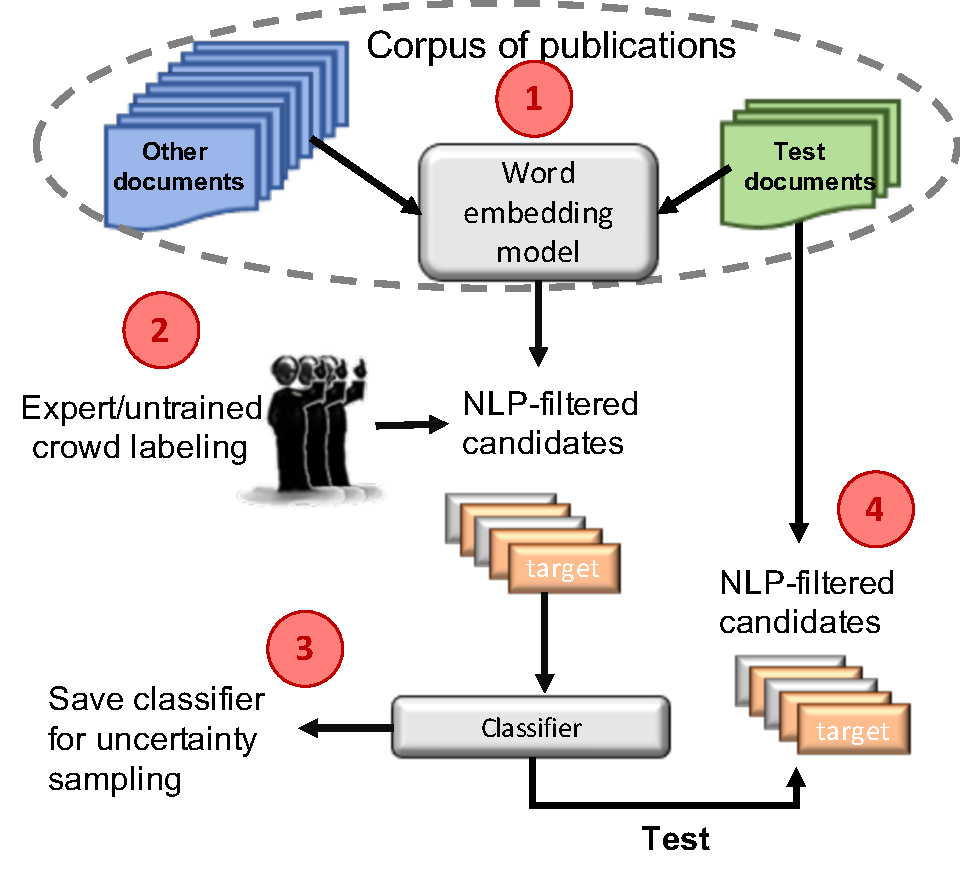
\includegraphics{figures/al_setup.pdf}}
\caption{\label{fig:current} The active learning experiment set up; we generate an unsupervised word embedding model using our entire corpus in 1), we propose NLP-filtered candidate entities to untrained and expert annotators in 2) before classifying their word vectors in 3). We save this classifier for uncertainty-based selection of labels for the next round of active learning. In 4), we test this word vector classifier on all NLP-filtered words from the test documents. 
%\logan{What are the blue docs? Why don't they have an arrow? Where do the NLP candidates for 2 come from?}
%\roselyne{They come from the entire pool of NLP-filtered candidates (excluding the test set, will make sure this is clear}
\ian{Could this fit in a single column?}
\ian{Here and in other figure, I find it confusing to have the description precede the number.}
}
\end{figure*}

\subsection{Active Learning Loop}
As we have no prior knowledge of the distribution of target entities in the vector space, 
we use multiple classifiers at each iteration of the active learning process. 
%\ian{What does it mean to ``save''?}\roselyne{we use,keep, mark? the classifier that will be used for sampling.}
We use the best performing classifier on the labeled candidates for subsequent maximum entropy-based uncertainty sampling. 
%\logan{You have neither defined nor motivated MEU, I think}\roselyne{See if you would add something to the previous strategies (UBS). That's where I've tried to define it, tell me if it's not clear}.
The requested labels are annotated by humans to serve as addition training data for the next learning iteration. 
We describes these steps in more details in the following sections.

\subsubsection{Untrained and Expert Labeling}
As explained in section~\ref{sect:background}, recognizing polymers can require more or less domain expertise.
We assign two domain experts to annotated candidates generated using our two maximum entropy-based uncertainty sampling (\textit{UBS} and \textit{Distance UBS}). 
Each expert annotates one strategy but we perform crosschecking for 10\% of the first batch of labels to get a measure of agreement between experts. 
%We confirm agreement between labels for all but 1 of the set of 20 candidates or an agreement of 95\%.
%\logan{The inter-relater score is a result, not part of the architecture}\roselyne{ok, don't remove, come back to this to make sure I add it later}
Experts simply approve or reject candidates using the web interface shown in Figure~\ref{fig:polyner},
a task that is far more efficient than reading and annotating words in text.
The interface
provides example sentences as context for ambiguous candidates,
and allows the expert to access the publication(s) in which a particular candidate
appears. % when desired.

Expert time is costly and we aim to reduce the cost of obtaining labels.
Therefore for our baseline of randomly sampled NLP-filtered nouns, we experiment with a two-phase review process.
Tokenization is one of the largest sources of error for scientific entities such as polymers, 
which contain characters such as `:', `(',
'\textendash', `,' etc. 
Tokenization can also generate incoherent tokens from text, equations, captions, and more.
Such obvious non-candidates can be fairly easily detected by non experts.
For example, an untrained human annotator may be able to recognize that `$d\Sigma/d\Omega)(Q$' is not a polymer name, and thus save time for the experts.
Hence, we assign two graduate student labelers to curate the candidates generated by the random sampling strategy, which are less likely to contain target entities.
First, the untrained labelers reject obvious non-candidates via the previously mentioned web interface. 
Next, one of our expert polymer scientists indicates, for each remaining
candidate, whether or not it is in fact a polymer referent and submits a final review.
While we first used this two-phase review process for the random strategy, 
we envision generalizing and leveraging humans with different expertise through multi-phase reviews for all strategies to further save costs.


\begin{figure}
\centering
\frame{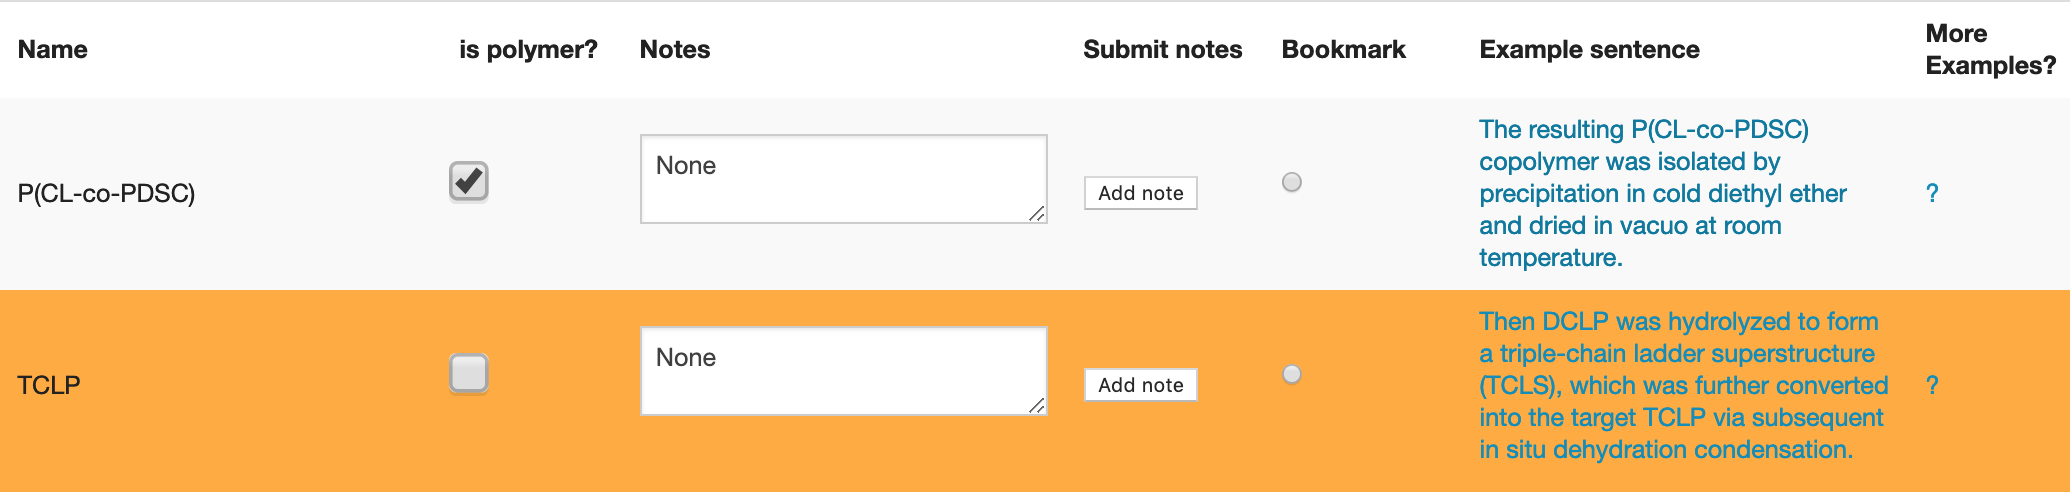
\includegraphics[trim=0in 0.1in 0.1in 0.in,clip,width=3.5in]{figures/expert_labeling.png}}
\caption{\label{fig:polyner} Web interface for expert review of candidates.
The expert indicates whether the name (col 1) is a polymer (col 2), 
providing notes if desired (col 3). 
Clicking on ``?'' delivers up to 25 more example sentences.
}
\end{figure}

\subsubsection{Classification or Candidate Discrimination}
We use multiple classifiers that we concurrently trained and test on the same data in steps 1, 2, and 3 of Figure~\ref{fig:current}.
The classifiers include the scikit-Learn~\cite{scikit-learn} implementations of Decision Tree (DT), Gradient Boosting (GB), K-Nearest Neighbor (KNN), Logistic Regression (LR), Linear Support Vector Machine (SVM), Naive Bayes (NB), and Random Forest (RF). 
%\logan{Something to consider for future: I've been nervous a long time about how we use so many models. How good is your grid search CV for these models? Many (KNN, SVM) are super sensitive to hyperparameters, and I'm worried we are testing 7 models badly and that we'd have better results with tuning 1 really well}
%\roselyne{Yes, this is definitely a lesson taken. I was just telling Kyle, I know exactly how I would change this experiment and others based on my experience now. Perhaps I need to say that in the discussion!}\roselyne{Added note to include in discussion}
Our goal here is to explore the word embedding space and determine which classifier(s) works best for detecting our scientific named entities.
As previously mentioned, we select%\ian{that word save again.} 
the \textit{best-performing} classifier on labeled candidates for subsequent uncertainty sampling.
When defining best performance, we prioritize recall, or retrieving a maximum of targets, over precise extraction.
In other words, extracting a higher number of targets potentially requiring additional curation is favored over obtaining fewer correct targets.
%\logan{Can you express this quantitatively?}\roselyne{I have favored recall, maybe I should just say that? better?}
In each case, we use the word embedding for each string as input features.
%\logan{Do you mean "use the word embedding for each word as input"? All word vectors should have the same dimensions}\roselyne{yes, they do, I want to indicate exactly that the valye of the dimensions word vector itself is used as features, I wasn't sure if the embedding for each word as input was clear enough.}




